
%%%% TODO: Adrien, this subsection has been already addressed in the previous subsection, so I commented it
%\subsection{Implementation of DVMS}
%
%A prototype of DVMS leveraging the \emph{peer actor} abstraction has been 
%developed. In addition we built two versions of the network overlay actor: one 
%working with Chord, and one working with the Vivaldi based overlay. This mean 
%that now DVMS is network overlay agnostic to, and thus can be used with either
%of the network overlay without requiring any modification in it's source code.
%
%The implementation is based on modern programming language and framework such as 
%\emph{Scala} and \emph{Akka framework}. Scala is a language that mixes object
%oriented programming with functional programming, it's compiler produces 
%\emph{Java bytecode} which can be run in any JVM environment. Combining Scala 
%with Akka enabled us to take advantage of advanced techniques for concurrent 
%programming such as \emph{future/promise} and \emph{actor model}, and to benefit
%from Java ease of deployment.
%


%\subsection{Grid'5000 experiments}

%\JP{Complete this section with more experimentation results.}

%\subsubsection{Objectives}
%The prototype has been tested with a various number of experiments conducted on
%the Grid'5000 testbed. 
The main objective of the experiments we conducted was to estimate the impact of locality on
the performance of a distributed scheduling algorithm. A significant portion of the
reconfiguration time is spent in live migration of virtual machines, which depends of
network parameters such as latency and bandwidth. One way to improve the performance of
distributed scheduling algorithms is to promote collaborations between close resources,
which can be reached by maximizing the ratio $nb\ intrasite\ migrations/nb\ migrations$.
%\[
%	\frac{number\ of\ intrasite\ migrations}{number\ of\ migrations}
%\]


\subsection{Experimental Protocol}

To compare our experiments, we implemented a dedicated injector that makes load changes of
VMs during a predefined time. VMs are launched on PMs in a round-robin manner, \ie each
PM hosts roughly the same number of VMs at the beginning. The experiment consists in
repeatedly changing target CPU loads of VMs. Every $t$ seconds, the injector that is
deployed on a dedicated node selects one VM and changes its CPU load according to a
Gaussian distribution. $t$ is a random variable that follows an exponential distribution
with rate parameter $\lambda$. The Gaussian distribution is defined by a mean ($\mu$) as
well as a standard deviation ($\sigma$) that are given at the beginning of the experiment.
%exponential and the Gaussian distributions previously described. 
The parameters are $\lambda=\mathit{Nb\_VMs}/300$ and $\mu=70$, $\sigma=30$.
Concretely, the load of each VM starts from 0\% and varies on average every 5
minutes in steps of 10 (with a significant part between 40\% and 100\% of CPU
usage). The duration of each experiment was set to 3600 seconds.

\begin{wrapfigure}{r}{0.38\textwidth}
 \begin{center}
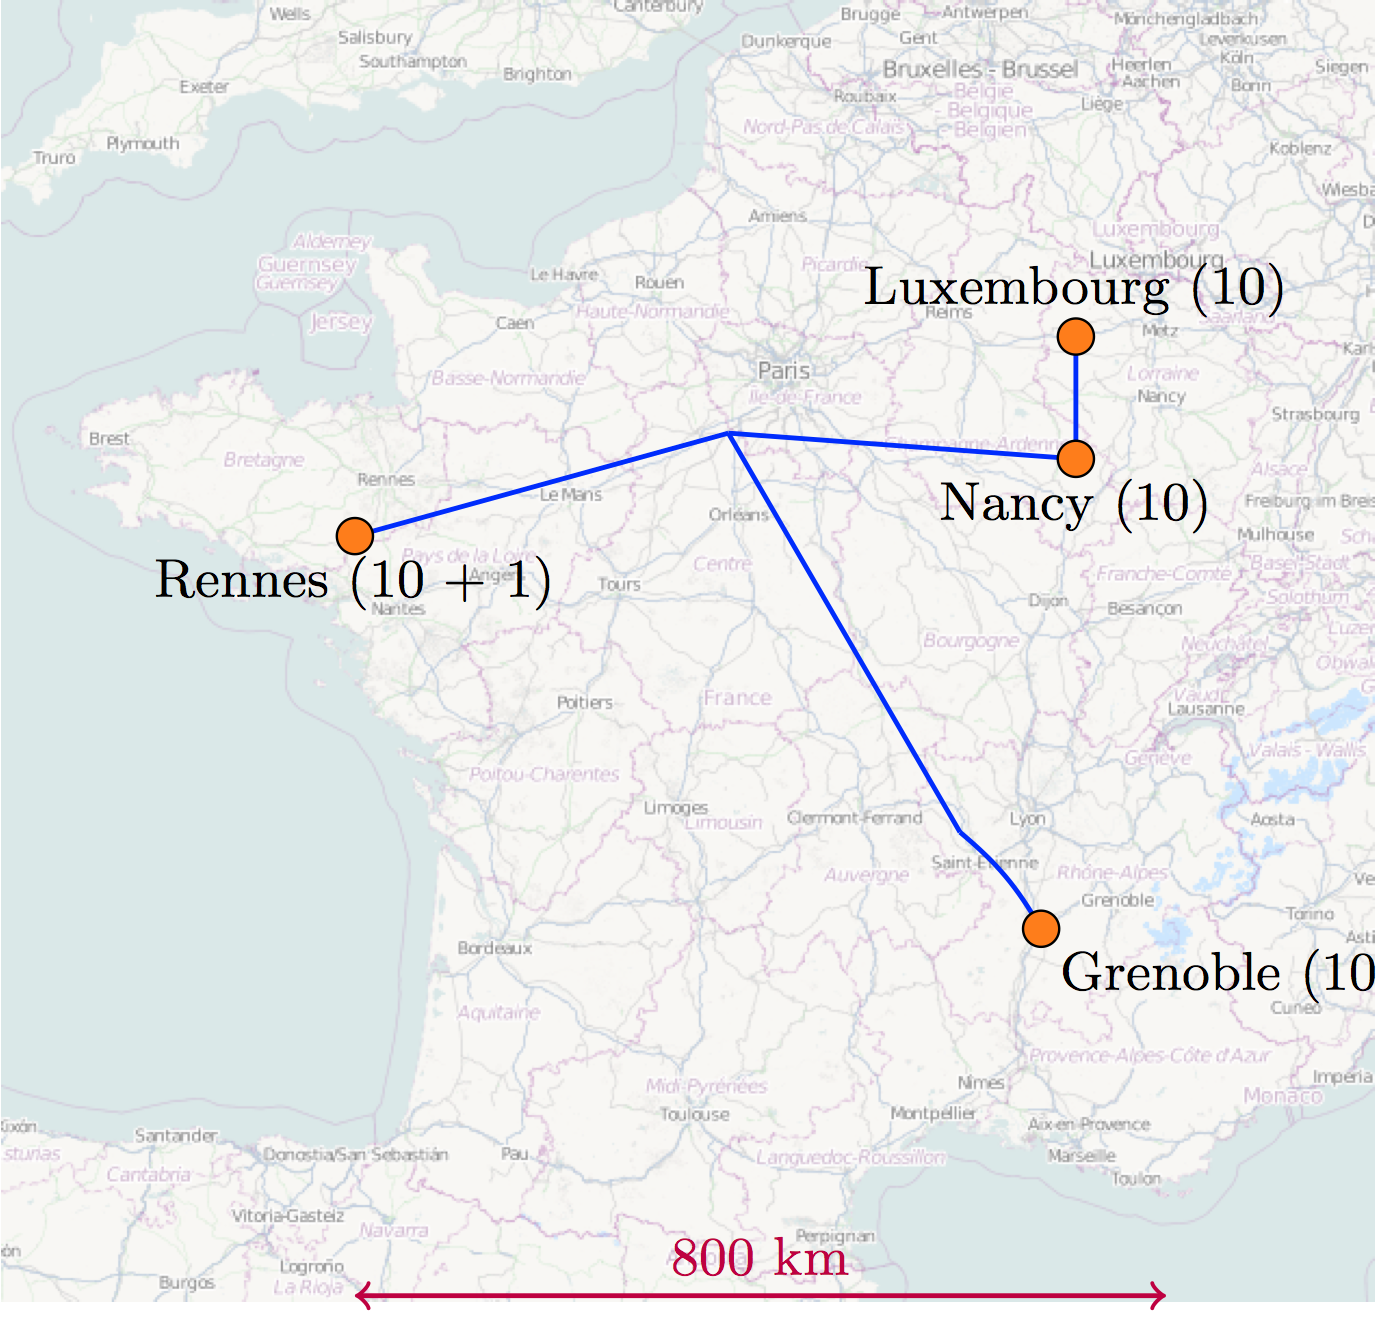
\includegraphics[width=0.38\textwidth]{./Figures/testbed.png}
\caption{Deployed testbed}
\label{fig:testbed}
\end{center}
\end{wrapfigure}

For each experiment, we booked 40 compute servers spread over 4 geographical sites (10
PMs per site) and 1 service server from the Grid'5000 testbed. The compute servers
were used to run VMs and DVMS while the service node runs the aforementioned
injector.
%
Each compute node was equipped with 8 cores and hosted a number of VMs
proportional to its number of CPU cores ($nb VM\ =\ 1.3\ \times\ nb\ cores)$, leading to
a global number of 416 VMs. Although such a number is rather small regarding the latest
experiments that have been performed on DVMS~\cite{quesnel:ispa2013}, our goal is not to
validate once again the scalability criteria but to focus on the locality aspect of such
an algorithm.
%\[
%	number\ of\ virtual\ machines\ =\ 1.3\ \times\ number\ of\ cores
%\]


\subsection{Results}

\subsubsection{Maximization of Intra-Site Migrations.}

Table~\ref{migration_table} compares the ratio between intra-site migrations and the total
number of migrations, using Chord or our locality-based overlay~(LBO) network. The results show that the impact of locality
is significant: Using LBO leads to an average number of 86.3\%
of intra-site migrations while using a Chord-based DVMS decreases this ratio to 49.6\%.

\begin{table}

  \begin{center}
    \begin{tabular}{|c|c|c|}   

      % <HEADER>
      \hline \multicolumn{1}{|p{3cm}|}{ }
       & \multicolumn{1}{|p{3cm}|}{\centering Chord }  & \multicolumn{1}{|p{3cm}|}{ \centering LBO}  \\
      % </HEADER>

      % <ROW 1> => Average
      \hline
      average & 0.496 & 0.863 \\
      % </ROW 1>

      % <ROW 2> => Min
      \hline
      minimum & 0.378 & 0.798 \\
      % </ROW 2>

      % <ROW 2> => Max
      \hline
      maximum & 0.629 & 0.935 \\
      % </ROW 2>

      \hline
    \end{tabular}
  \end{center}
  \caption{\label{migration_table} Comparison of intra-site migrations ratio
    using DVMS/Chord and DVMS/LBO.}
  \vspace{-0.3cm}
\end{table}


\subsubsection{Dynamic Clustering.}

During our investigation of the results brought about LBO, we noticed that many of the
inter-site migrations were performed between Luxembourg and Nancy sites.
In Table~\ref{latency_table}, it is noticeable that Luxembourg and Nancy have a latency that is significantly
below usual inter-site latencies (Nancy and Luxembourg are separated by only 100 kilometers),
while Rennes and Grenoble have almost the same latency with all their respective remote sites.
Indeed, servers located in Luxembourg and Nancy are more likely to collaborate with each other, while those located
on Rennes and Grenoble will find collaborators regardless of their location. This explains
why many of the inter-site migrations were performed between Luxembourg and Nancy.
This means that LBO enabled DVMS to learn which site is more interesting to perform VM
migration. Promoting low latency inter-site collaboration made many inter-site
migrations acceptable compared to those executed by the Chord version.


\begin{table}[t!]

  \begin{center}
    \begin{tabular}{|c|c|c|c|c|}   

      % <HEADER>
      \hline \multicolumn{1}{|p{2cm}|}{ } & \multicolumn{1}{|p{2cm}|}{\centering Grenoble }  & \multicolumn{1}{|p{2cm}|}{\centering Luxembourg } & \multicolumn{1}{|p{2cm}|}{\centering Nancy }& \multicolumn{1}{|p{2cm}|}{\centering Rennes } \\
      % </HEADER>

      % <ROW 1> => Grenoble
      \hline
      Grenoble & 0.09 ms & 16.55 ms & 14.24 ms & 15.92 ms \\
      % </ROW 1>

      % <ROW 2> => Luxembourg
      \hline
      Luxembourg &  & 0.17 ms & 2.70 ms & 13.82 ms \\
      % </ROW 2>

      % <ROW 3> => Nancy
      \hline
      Nancy & &  & 0.27 ms & 11.42 ms \\
      % </ROW 3>

      % <ROW 4> => Rennes
      \hline
      Rennes &  &  &  & 0.23 ms \\
      % </ROW 3>

      \hline
    \end{tabular}
  \end{center}
  \caption{\label{latency_table} Latency measured between sites.}
\end{table}


% \vspace{-1.0cm}


% \vspace{-1.3cm}

\subsubsection{Reactivity.}
\begin{table}[t!]

  \begin{center}
    \begin{tabular}{|c|c|c|}   

      % <HEADER>
      \hline \multicolumn{1}{|p{3cm}|}{ }
       & \multicolumn{1}{|p{3cm}|}{\centering Chord }  & \multicolumn{1}{|p{3cm}|}{ \centering LBO}  \\
      % </HEADER>

      % <ROW 1> => Number of sites
      \hline
      average number of sites involved & 1.645 & 1.082 \\
      % </ROW 1>

      % <ROW 2> => Duration
      \hline
      average scheduling duration (msec) & 154.63 & 98.50 \\
      % </ROW 2>

      \hline
    \end{tabular}
  \end{center}
  \caption{\label{partitions_table} Comparison of partitions metrics
    using DVMS/Chord and DVMS/LBO.}
  \vspace{-0.3cm}
\end{table}

% \vspace{-1.0cm}

Table~\ref{partitions_table} depicts metrics that allow for an objective 
comparison of the efficiency of both overlay networks. In addition of reducing 
the number of inter-site migrations, the side effect of using the LBO is to 
reduce the solving time: partition duration is 46\% lower than that encountered 
with Chord. This result is consistent with the fact that with our locality-aware
overlay, the number of sites that are involved in partitions becomes very close 
to one. Indeed collaborating with closer nodes allows exchanging information between
nodes of the partition much faster, thus increasing once again the reactivity
of the system.
%% TODO (ici ca aurait ete bien de donner un odre de grandeur sur la difference entre le temps de migration intra-site vs inter-sites pour deux VMS de meme classe (i.e. qui ont la meme memory intensity, celle défini dans le code de l'injector). 

% 
